\chapter{Localization}

\section{Peak detection}

The received signal, consisting of summed delayed signals, cross-correlated by every anchor. If the signal is not reflected the peak in cross-correlation would be obvious. But because by the introduction of noise and water reflections a higher rate of similar peaks appear. To suppress these effects a CA-FAR Algorithm \cite{rohling11} is applied to only detect the first reflected peak resulting in lower false alarms of peaks. \\
CA-FAR works by using multiple values intervals. The most outer one could be described as a train bin and is used to get an estimation of the signals noise. Especially CA-FAR uses averaging to estimate the noise by measured cells. The bordering bin, defined as the guard cells, is used to reduce self-interference of the peaks. Thus, increasing window sizes $W$ results in better noise estimating but overall detectability is still limited by the sample rate  \cite{rohling11}\cite{radarbasics}. By knowledge of measured peak widths a optimal guard interval can be figured.\\
The calculated threshold is than scaled by factor $S$ depending on a formula based on the false alarm rate $\eta$. The higher the false alarm rate, the weaker high amplitude peaks gets included by the estimated threshold \ref{eq:cff}.\\

%Because Cell Averaging shows not satisfactory results in sensitive multi targets examples, the noise estimation could be enhanced by a sorting average applied to the %train interval. That principle is defined as CO-FAR \cite{rohling11}. 
%\begin{center}
%	\begin{tabular}{|c|c|}
	%			\hline
	%			candidate sample & $i$\\
	%			\hline
	%			guard interval (half) & $\mathcal{G}$ \\
	%			\hline
	%			train interval (half) & $\mathcal{T}$ \\
	%			\hline
	%			false alarm rate & $\eta$\\
	%			\hline
	%		\end{tabular}
%	\linebreak
%\end{center}
%
%\begin{equation}
%	Threshold(i)_x=
%	\cfrac{\alpha}{2\mathcal{T}}
%	\left[ \sum_{j=i-\left( \mathcal{G}+\mathcal{T}\right) }^{i+\left( \mathcal{G}+\mathcal{T}\right)}x(j) - \sum_{j=i-\mathcal{G}}^{i+\mathcal{G}}x(j) \rigbest NAht] 
%	\label{eq:cft}
%\end{equation}
\begin{equation}
	S=2W\left( \eta^{-1/{2W}}-1\right) 
	\label{eq:cff}
\end{equation}

\begin{figure}[h]
	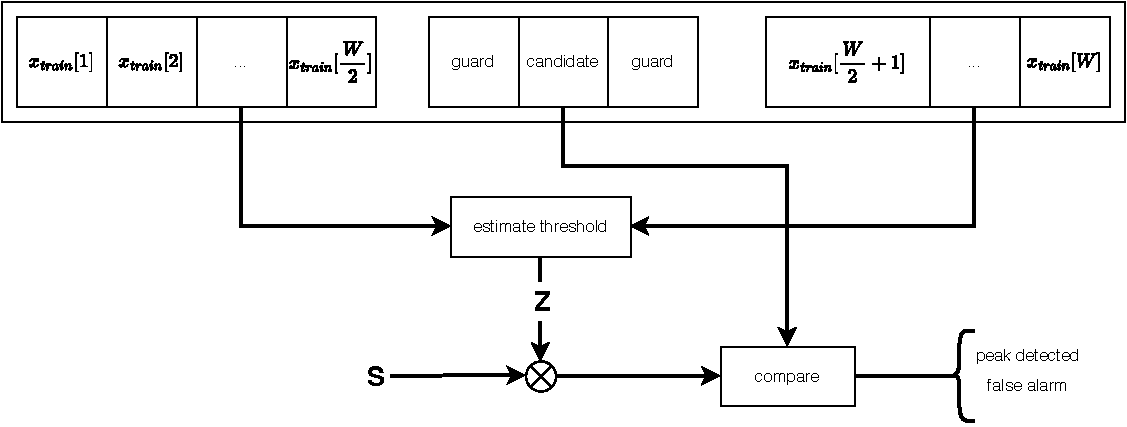
\includegraphics[width=\linewidth]{images/peakdet}
	
	\caption{CFAR threshold peak detection procedure \cite{rohling11}}
	\label{fig:simsig}
\end{figure}

\begin{equation}
	T=S\cdot Z,~~~Z_{CA}=\sum_{i=1}^{W}\dfrac{1}{W}x_{train}
\end{equation}
%\section{Explicit Position calculation}
%
%The initial condition for the localization are four anchors $S_i$ with thir coordinates $\{x_i,y_i,z_i\}$ and the target $S$ which is to be located. By multiplying relative delays by the speed of sound $c$ which is approximately set to $1500\,\frac{m}{s}$, the distance $d_{ij}$ between the reference anchor $S_0$ and $S_i$ is calculated.\\
%\begin{equation}
%	d_{ij}=c\cdot\tau_{ij}=c\cdot (t_i-t_j),~~~\text{absolute delays } t_k,~k\in \{0,1,2,3\}
%\end{equation}
%By these values a Matrix $A$ and vector $\vec{b}$ is created. Thus, a System $A\cdot \vec{x}=\vec{b}$ is established. This linear system can be solved by using the inverse method if Matrix $A$ has full rank. Otherwise least squared can be used but yields undesirable results. In three dimensional Space five anchors are needed for full rank. The solution $\vec{x}$ are the coordinates $\{x,y,z\}$ of the target $S$ \cite{yang11}.
%
%\begin{equation}
%	A=\left[
%	\begin{array}{cccc}
%		x_0-x_1 & y_0-y_1 & z_0-z_1 & d_{01}\\
%		x_0-x_2 & y_0-y_2 & z_0-z_2 & d_{02}\\
%		x_0-x_3 & y_0-y_3 & z_0-z_3 & d_{03}\\
%		x_0-x_4 & y_0-y_4 & z_0-z_4 & d_{04}\\
%	\end{array}
%	\right]
%\end{equation}
%\begin{equation}
%	\vec{b}=\cfrac{1}{2}\left[
%	\begin{array}{c}
%		x_0^2-x_1^2+y_0^2-y_1^2+z_0^2-z_1^2+d_{01}^2\\
%		x_0^2-x_2^2+y_0^2-y_2^2+z_0^2-z_2^2+d_{02}^2\\
%		x_0^2-x_3^2+y_0^2-y_3^2+z_0^2-z_3^2+d_{03}^2\\
%		x_0^2-x_4^2+y_0^2-y_4^2+z_0^2-z_4^2+d_{04}^2\\
%	\end{array}
%	\right]
%	,~~~
%	\vec{x}=\left[
%	\begin{array}{c}
%		x\\
%		y\\
%		z\\
%		||S-S_0||_2\\
%	\end{array}
%	\right]
%\end{equation}
%Theoretically an system $A$ of lower rank can be solve by least squares. Having said this, positions calculated by that approach could not satisfy the demands of 3D localization.
%
%\begin{equation}
%	\vec{x}=(A^T A)^{-1} A^T\vec{b}
%\end{equation}

\section{hyperbolic intersection localization method}

The initial condition for the localization are four anchors $S_i$ with thir coordinates $\{x_i,y_i,z_i\}$ and the target $S$ which is to be located. By multiplying relative delays by the speed of sound $c$ which is approximately set to $1500\,\frac{m}{s}$, the distance $d_{ij}$ between the reference anchor $S_0$ and $S_i$ is calculated  \cite{yang11}.\\
\begin{equation}
	d_{ij}=c\cdot\tau_{ij}=c\cdot (t_i-t_j),~~~\text{absolute delays } t_k,~k\in \{0,1,2,3\}
\end{equation}
\begin{equation}
	x_{ji}:=x_j-x_i,~~~~~
	y_{ji}:=y_j-y_i,~~~~~
	z_{ji}:=z_j-z_i~~~~~
\end{equation}
Every TDOA estimate creates hyperbolic curves which anchors is placed at its foci. 
By rearranging the derivation of hyperbola intersections the following substitutes can be defined \cite{bucher02}. 
\begin{equation}
	{A}=\cfrac{d_{02}x_{10}-d_{01}x_{20}}{d_{01}y_{20}-d_{02}y_{10}},~~~
	{B}=\cfrac{d_{02}z_{10}-d_{01}z_{20}}{d_{01}y_{20}-d_{02}y_{10}}
\end{equation}	
(The complete formula is inside the appendix)
%\begin{equation}
%	{C}=\cfrac{d_{02}\left(d_{01}^2+x_0^2-x_1^2+y_0^2-y_1^2+z_0^2-z_1^2\right)-d_{01}\left(d_{02}^2+x_0^2-x_2^2+y_0^2-y_2^2+z_0^2-z_2^2\right)}{2\left(d_{01}y_{20}-d_{02}y_{10}\right)}
%\end{equation}	
%
%\begin{equation}
%	{D}=\cfrac{d_{23}x_{12}-d_{21}x_{32}}{d_{21}y_{32}-d_{23}y_{12}},~~~
%	{E}=\cfrac{d_{23}z_{12}-d_{21}z_{32}}{d_{21}y_{32}-d_{23}y_{12}}
%\end{equation}	
%\begin{equation}
%	{F}=\cfrac{d_{23}\left(d_{21}^2+x_1^2-x_1^2+y_1^2-y_1^2+z_0^2-z_1^2\right)-d_{21}\left(d_{23}^2+x_1^2-x_2^2+y_1^2-y_2^2+z_1^2-z_2^2\right)}{2\left(d_{21}y_{32}-d_{23}y_{12}\right)}
%\end{equation}	
%
%\begin{equation}
%	{G}=\cfrac{{E}-{B}}{{A}-{D}},~~~
%	{H}=\cfrac{{F}-{C}}{{A}-{D}},~~~
%	{I}={A}\cdot {G}+{B},~~~
%	{J}={A}\cdot {H}+{C}
%\end{equation}	
%
%\begin{equation}
%	{K}=d_{02}^2+x_0^2-x_2^2+y_0^2-y_2^2+z_0^2-z_2^2+2x_{20}{H}+2y_{20}{J}
%\end{equation}	
%
%\begin{equation}
%	{L}=2\left(x_{20}{G}+y_{20}{I}+z_{20}\right)
%\end{equation}	
%
%\begin{equation}
%	{M}=4d_{02}^2\left({G}^2+{I}^2+1\right)-{L}^2
%\end{equation}	
%
%\begin{equation}
%	{N}=8d_{02}^2\left[{G}\left(x_0-{H}\right)+{I}\left(y_0-{J}\right)+z_0\right]+2{L}\cdot{K}
%\end{equation}	
%
%\begin{equation}
%	{O}=4d_{02}^2\left[\left(x_0-{H}\right)^2+\left(y_0-{J}\right)^2+z_0^2\right]-{K}^2
%\end{equation}	

A downside of this approach is the uncertainty of position $z$. Thus, additional information on bounds is necessary. The target won't get above sea level. Consequently, at least one boundary $z_{surface}$ which acts like a maximum can be set. The minimum value $z_{ground}$ can be assumed as the lowest position achievable underwater. 
\begin{equation}
	z_{a,b}=\cfrac{{N}}{2{M}}\pm\sqrt{\left(\cfrac{{N}}{2{M}}\right)^2-\cfrac{{O}}{{M}}}
\end{equation}	

\begin{equation}
	z=\min\left\{\max\left\{z_a,~z_b,~z_{surface}\right\},~z_{ground}\right\}
\end{equation}	

One other solution to this issue is to utilize information about our previous location $z'$. Specifically, we can calculate the distance between our current position and the two potential candidates for the next estimate of z, and choose the candidate with the shorter distance.
\begin{equation}
	z=\begin{cases}
		z_a & \text{if }\abs{z_a-z'}<\abs{z_b-z'}\\
		z_b & \text{else}
	\end{cases}
\end{equation}	

The resulting x and y values of our target can then be calculated by the following formula using the selected $z$.

\begin{equation}
			\vec{x}
	=\left[
	\begin{array}{c}
		x\\
		y\\
		z
	\end{array}
	\right]
=\left[
	\begin{array}{c}
		{G}z+{J}\\
		{I}z+{H}\\
		z
	\end{array}
	\right]
\end{equation}	

\section{Localization Simulation}
In preparation for the field testing, several 3-dimensional space paths were simulated, wherein the generated points formed a helical curve that expanded in the z-direction. The positions of four anchors were utilized to calculate the corresponding Time Difference of Arrival (TDOA) values, which were subsequently incorporated into the localization algorithm. Multiple runs, utilizing varying SNR's and watermark channels were conducted to evaluate the performance of the peak detection method.\\
\begin{equation}
	\vec{x}_{\phi}(\alpha,\beta)
	=\left[
	\begin{array}{c}
		x=\alpha\cdot\sin{\phi}+\beta\\
		y=\alpha\cdot\cos{\phi}+\beta\\
		z=[|\phi|,-1)
	\end{array}
	\right]
\end{equation}

\begin{equation}
	-
\end{equation}

\section{Localization field testing}

The field test was carried out on a shore. Two hydrophones were placed one meter under sea level. The anchors A and B were placed with a distance of $4.1\,m$. Anchor B was placed $10.74\,m$ from the recieving hydrophone. The at that time under water measured speed of sound was $1430.3\,\frac{m}{s}$.